\documentclass[conference]{IEEEtran}
\IEEEoverridecommandlockouts

\usepackage{cite}
\usepackage{amsmath,amssymb,amsfonts}
\usepackage{algorithm}
\usepackage{algorithmic}
\usepackage{graphicx}
\usepackage{textcomp}
\usepackage{xcolor}
\usepackage{booktabs}
\usepackage{array}
\usepackage{tabularx}
\usepackage{tikz}
\usetikzlibrary{arrows.meta,positioning,shapes.geometric,fit,backgrounds}
\usepackage{pgfplots}
\pgfplotsset{compat=1.16}

% Float placement tuning to prevent float-only pages
\renewcommand{\floatpagefraction}{0.85}
\renewcommand{\textfraction}{0.10}
\renewcommand{\topfraction}{0.90}
\renewcommand{\bottomfraction}{0.70}
\setlength{\floatsep}{3.5pt plus 1pt minus 1pt}
\setlength{\textfloatsep}{4.5pt plus 1pt minus 1pt}
\setlength{\intextsep}{3.5pt plus 1pt minus 1pt}
\setlength{\abovecaptionskip}{2.5pt}
\setlength{\belowcaptionskip}{1pt}
\setcounter{topnumber}{4}
\setcounter{bottomnumber}{2}
\setcounter{totalnumber}{6}

\begin{document}

\title{Temporally Grounded Agentic Retrieval-Augmented Generation with Deterministic Safety Enforcement for Disaster Situational Awareness}

\author{
\IEEEauthorblockN{
Christopher Aseer J Albert\textsuperscript{1},
Prisha Andrew Bhosale\textsuperscript{2},
Ashutosh Monish Bhonsle\textsuperscript{3},\\
Chaitanya Vijaykumar Mahamuni\textsuperscript{4}, and
Dakshayani G\textsuperscript{5}
}
\IEEEauthorblockA{
\textsuperscript{1,2,3,5}\textit{Department of Computer Engineering, Fr. C Rodrigues Institute of Technology, Vashi, India}\\
\textsuperscript{4}\textit{Electronics and Telecommunication Engineering, University of Mumbai, Mumbai, India}\\
\textsuperscript{1}\texttt{christpheraseer5080@gmail.com}, \textsuperscript{2}\texttt{prisha.bhosale22@gmail.com},\\
\textsuperscript{3}\texttt{bhonsle.ashutosh@gmail.com}, \textsuperscript{4}\texttt{chaitanyamahamuni91@gmail.com},\\
\textsuperscript{5}\texttt{dakshayani@fcrit.ac.in}
}
}

\maketitle

\begin{abstract}
Operational disaster situational awareness demands synthesizing time-critical information across asynchronous crisis microblogs, real-time hydrologic and meteorological telemetry, and official emergency response doctrine. Standard retrieval-augmented generation (RAG) paradigms exhibit critical operational failure modes in safety-critical environments: they conflate historical incident archives with active field conditions, fail to ingest live sensor fluctuations, and lack deterministic boundaries against hazardous directives. This paper presents an agentic RAG framework designed for disaster response, integrating two core mechanisms: Temporal Grounding Injection (TGI), which stratifies evidence into rolling categorical recency tiers, and a Deterministic Safety Enforcement Layer (DSEL), which executes pattern-based directive screening, citation verification, and fail-closed alert gating. An autonomous reasoning agent coordinates an eight-tool registry interfacing with live river gauges, meteorological forecasts, seismic catalogs, and official emergency response doctrine. On the 200-query DAB-200 benchmark, the system achieves 0.0915 keyword-F1 on held-out evaluations, compared to 0.0657 for static RAG. On a two-sided temporal stress test, TGI eliminates false evacuation directives on safe live readings (0/36 vs. 10/36 for the ungrounded agent), while exhibiting an 8.3\% miss rate on critical flood stages. Adversarial stress testing demonstrates that rule-based screening reduces unsafe directives from 21.4\% to 0.8\%, establishing a verifiable, fail-closed operational baseline for computer-assisted emergency situational awareness.
\end{abstract}

\begin{IEEEkeywords}
Agentic retrieval-augmented generation, disaster situational awareness, temporal grounding, deterministic safety enforcement, large language models, hallucination mitigation.
\end{IEEEkeywords}

%==========================================================
%==========================================================
\section{Introduction}
Natural and anthropogenic disasters---including flash floods, earthquakes, wildland fires, and hazardous chemical releases---cause severe casualties and damage critical infrastructure globally \cite{undrr}. Timely emergency response depends on operational situational awareness: a verified, spatio-temporally bounded picture of hazard severity and population vulnerability \cite{endsley,aboualola2023}. Emergency operations centers (EOCs) must assemble this awareness under severe time pressure from heterogeneous streams: satellite and UAV imagery, crowdsourced microblogs, in-situ IoT sensors, and official response doctrine \cite{crisismmd,aboualola2023}.

Recent AI advances have accelerated specialized disaster tasks, including aerial damage assessment \cite{singh}, crisis social-media filtering \cite{olteanu2015,dinani}, and emergency reporting \cite{cantini}. However, autoregressive language models generate plausible but factually erroneous or operationally fatal directives under distributional shift \cite{ji,yu2024}. In safety-critical contexts, ungrounded advice on evacuation corridors, structural stability, or water safety carries severe physical consequences. Standard retrieval-augmented generation (RAG) \cite{lewis} conditions generation on external documents, yet exhibits three fundamental failure modes in dynamic disaster operations: temporal conflation of archival and active reports, telemetry blindness due to static text indexing, and the absence of deterministic boundaries against hazardous output.

Formally, an emergency query $q$ issued at time $t_q$ for region $\ell$ operates over a corpus $\mathcal{D} = \mathcal{D}_{\mathrm{doc}} \cup \mathcal{D}_{\mathrm{hist}} \cup \mathcal{D}_{\mathrm{live}}$, where document chunks $x \in \mathcal{D}$ carry observation timestamps $t_x$. A response $\hat{y}$ exhibits temporal conflation when it asserts active conditions derived exclusively from archival records $x \in \mathcal{D}_{\mathrm{hist}}$ ($t_q - t_x \gg \Delta t$, with $\Delta t = 72$~h aligned with FEMA operational cycles) despite contradictory live telemetry $x' \in \mathcal{D}_{\mathrm{live}}$. Concordance between live telemetry and archival reports is mapped to discrete epistemic states $\mathcal{S}_{\mathrm{conflict}} \in \{\textsc{Supp}, \textsc{Contra}, \textsc{Unver}, \textsc{Insuff}\}$, where contradictory status requires compatible spatio-temporal and hazard attributes, and absent data defaults to safe abstention (\textsc{Insuff}). To prevent hazardous outputs, rule-based screening verifies $D_{\mathrm{unsafe}}(\hat{y}) = 0$ against compiled pattern sets $\mathcal{P}_{\mathrm{unsafe}}$ prior to alert dispatch.

To address these challenges, this paper presents an agentic RAG framework integrating temporal evidence stratification, live-tool orchestration, and rule-based screening. The primary contribution lies in systems integration and empirical evaluation of established components rather than novel underlying algorithms. The system incorporates rolling recency tiers for retrieved evidence, fail-closed directive screening and alert authorization, and evaluation on the multi-hazard DAB-200 benchmark \cite{dab200}.

We address three research questions:
\begin{enumerate}
    \item[\textbf{RQ1:}] Does explicit temporal evidence tiering reduce reliance on archival disaster reports when live sensor telemetry is available?
    \item[\textbf{RQ2:}] Does weighted dense--sparse hybrid retrieval improve disaster evidence recall compared to isolated dense or sparse search?
    \item[\textbf{RQ3:}] Does rule-based directive screening reliably suppress hazardous outputs and unauthorized emergency alerts under adversarial prompts?
\end{enumerate}

The remainder of this paper is organized as follows: Section~II surveys related work; Section~III details system architecture and mechanisms; Section~IV outlines the experimental setup; Section~V analyzes empirical results; Section~VI discusses limitations; and Section~VII concludes.

%==========================================================
\section{Related Work}
\subsection{Crisis Informatics and Multimodal Disaster Intelligence}
Crisis informatics has built a substantial empirical foundation. CrisisMMD \cite{crisismmd} provides paired tweet-image records across seven natural disasters; Rezk et al.\ \cite{rezk2023} apply multimodal channel attention for crisis classification; CrisisLex \cite{olteanu2014} supplies a 26-event microblog corpus with lexical relevance labels; and HumAID \cite{humaid} offers fine-grained humanitarian action categories across 19 events. More recently, Yu et al.\ \cite{yu2025} tackle open-world disaster event identification and Kim et al.\ \cite{kim2025} integrate multimodal streams for real-time event classification. These systems confirm that disaster-relevant signals can be reliably extracted from social and image feeds. What they do not provide is a mechanism for deciding whether a classified report reflects current field conditions, reconciling it against concurrently updated sensor telemetry, or constraining how that decision translates into an authorized response action.

\subsection{Temporal Information Retrieval and Evidence Freshness}
Sensor networks such as USGS stream gauges and seismic accelerometers supply primary observational evidence. Readings carry calibration uncertainty, spatial coverage limits, and ingestion latency \cite{manuel2024}. These are physical constraints, not defects of the data format. On the retrieval side, Piryani et al.\ \cite{piryani2023} survey temporal question answering and document systematic degradation when event time, observation time, and retrieval time are conflated. The CrisisFACTS track \cite{crisisfacts} benchmarks multi-stream summarization under evolving event timelines, and FreshQA \cite{freshqa} measures QA accuracy against world-knowledge that changes after model training. Together, these studies show that timestamp metadata alone is not sufficient: when periodically refreshed telemetry must be compared against archival incident reports, the system requires explicit tier separation and comparability constraints, not just recency labels.

\subsection{Agentic RAG and Tool-Orchestrated Reasoning}
ReAct \cite{react} established the interleave of chain-of-thought reasoning steps with environment observations, grounding generation in retrieved or tool-fetched evidence. LangGraph \cite{langgraph} extends this to stateful directed graphs for multi-actor workflows. Self-RAG \cite{selfrag} introduces learned reflection tokens for retrieval necessity and faithfulness; Corrective RAG \cite{crag} adds a lightweight relevance assessor that triggers web search on retrieval failure. Zhang et al.\ \cite{zhang2024} construct a knowledge graph over earthquake emergency doctrine and demonstrate that structured retrieval improves factual grounding on domain queries. Each of these advances strengthens retrieval quality or tool use. None defines a hard contractual boundary between the reasoning process and the alert-dispatch output. Producing a warning or evacuation order is a consequential, non-retractable action; it demands a gate that is not conditional on the stochastic behaviour of the generation model.

\subsection{Safety Guardrails and Runtime Verification}
Hallucination mitigation approaches fall broadly into retrieval grounding, chain-of-verification, and external guardrails \cite{ji,yu2024}. RAGAS \cite{ragas} automates faithfulness and relevance evaluation via LLM judges, providing a scalable audit layer. NeMo Guardrails \cite{nemoguardrails} governs conversational flows through Colang specifications. Llama Guard \cite{inan2023} applies a classifier trained on safety taxonomies to flag harmful outputs. These systems target general conversational safety objectives. They do not carry geospatial or temporal awareness of physical hazard states, and they were not designed to function as fail-closed authorization gates for public emergency alerts. Our screening layer is narrower in scope and makes no claim of superiority on latency or general safety coverage; it adds deterministic pattern interception and a physical-condition authorization predicate specifically at the alert-dispatch boundary, with residual violations reported empirically in Section~V.

\begin{table}[t]
\caption{Comparative Summary of Related Frameworks}
\label{tab:lit}
\centering
\scriptsize
\setlength{\tabcolsep}{2pt}
\begin{tabular*}{\columnwidth}{@{\extracolsep{\fill}}lcccc@{}}
\toprule
Approach & Temporal & Live & HUC-10 & Fail-Closed \\
         & Tiers & Telemetry & Gating & Alert Gate \\
\midrule
Crisis Informatics \cite{crisismmd,humaid} & \texttimes & \texttimes & \texttimes & \texttimes \\
Temporal QA \cite{piryani2023,freshqa} & \checkmark & \texttimes & \texttimes & \texttimes \\
Sensor Fusion \cite{manuel2024} & \texttimes & \checkmark & \texttimes & \texttimes \\
Agentic RAG \cite{react,selfrag,crag} & \texttimes & \texttimes & \texttimes & \texttimes \\
Safety Guardrails \cite{nemoguardrails,inan2023} & \texttimes & \texttimes & \texttimes & \texttimes \\
\midrule
\textbf{This work} & \checkmark & \checkmark & \checkmark & \checkmark \\
\bottomrule
\end{tabular*}
\end{table}

The gap across all prior categories is consistent: no existing system jointly addresses temporal evidence validity, live telemetry integration, hydrological catchment gating, and non-stochastic alert authorization. Table~\ref{tab:lit} maps these dimensions. The following section presents the system architecture and operational mechanisms.

%==========================================================
%==========================================================
\section{Methodology}

\subsection{System Architecture}
Fig.~\ref{fig:arch} presents the four-plane architecture. The \textit{Data Plane} ingests heterogeneous streams, extracts timestamps via Snowflake bitwise shifts, and enforces geospatial boundary filtering. The \textit{Agentic Reasoning Plane} executes a LangGraph ReAct cycle that coordinates an 8-tool registry and hybrid retrieval engine. The \textit{Safety Control Plane} intercepts candidate outputs through the 4-tier DSEL pipeline prior to EOC delivery. The \textit{Observability and Audit Plane} maintains an append-only JSONL ledger for post-incident provenance replay.

\begin{figure*}[!t]
\centering
\resizebox{0.58\textwidth}{!}{%
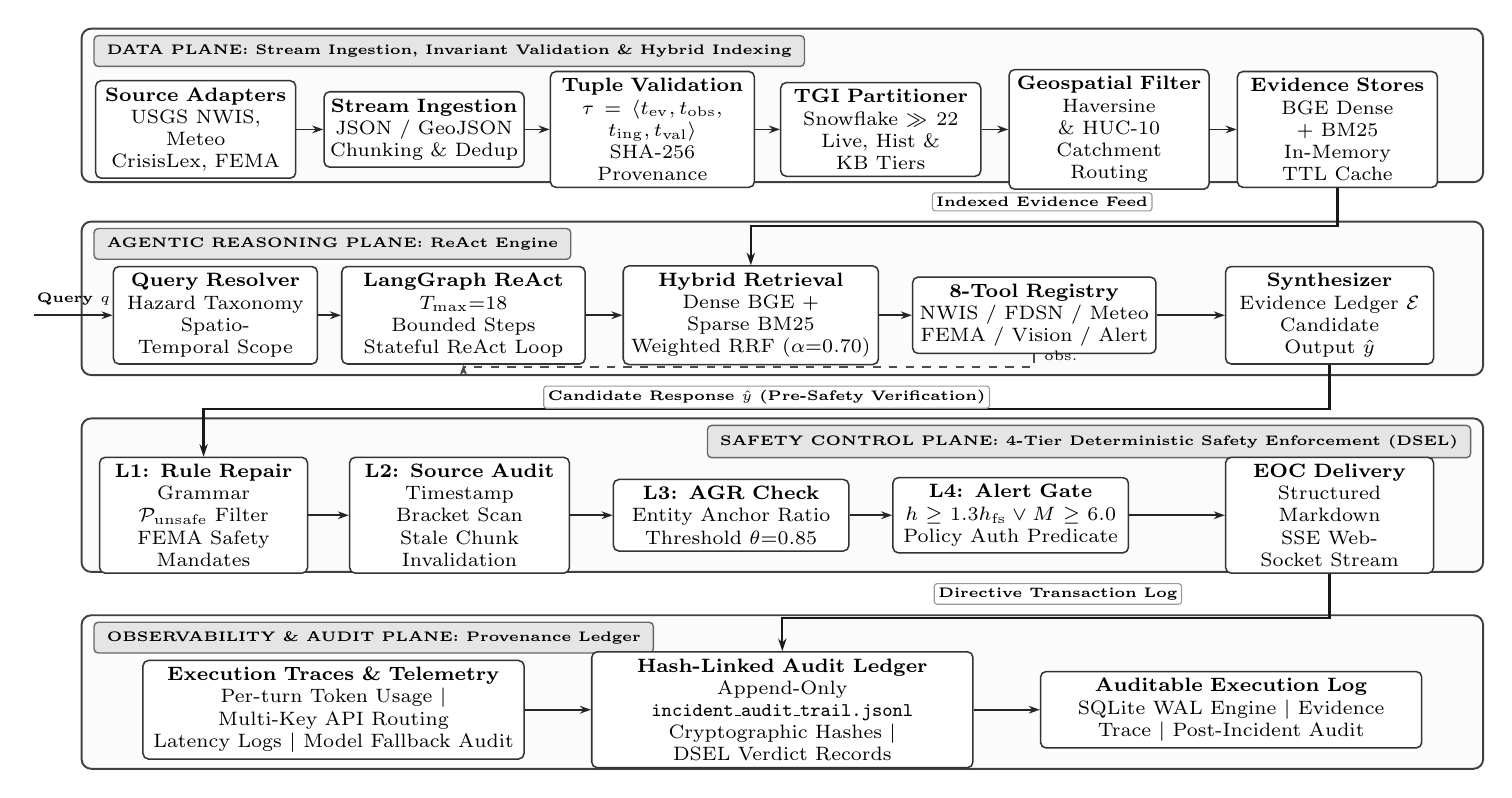
\begin{tikzpicture}[
  x=1cm, y=1cm, font=\scriptsize,
  plane/.style={draw=black!75, fill=gray!3, line width=0.7pt, rounded corners=3.5pt},
  tab/.style={draw=black!60, fill=gray!20, line width=0.5pt, rounded corners=1.5pt, font=\tiny\bfseries},
  comp/.style={draw=black!80, fill=white, line width=0.55pt, rounded corners=2pt,
               align=center, inner xsep=2pt, inner ysep=2.5pt, minimum height=0.88cm, font=\scriptsize},
  arr/.style={-{Stealth[length=4pt,width=2.8pt]}, line width=0.65pt, draw=black!85},
  dashedarr/.style={-{Stealth[length=4pt,width=2.8pt]}, line width=0.65pt, draw=black!70, dashed},
  interarr/.style={-{Stealth[length=4.5pt,width=3pt]}, line width=0.8pt, draw=black!90}
]

%% Total width: 17.80 

%% =========================================================================
%% PLANE 1: DATA INGESTION & STORAGE PLANE  (y: 7.45 -> 9.40)
%% =========================================================================
\draw[plane] (0, 7.45) rectangle (17.80, 9.40);
\node[tab, anchor=north west] at (0.15, 9.32)
  {\,DATA PLANE: Stream Ingestion, Invariant Validation \& Hybrid Indexing\,};

\node[comp, text width=2.40cm] (src)   at ( 1.45, 8.12)
  {\textbf{Source Adapters}\\USGS NWIS, Meteo\\CrisisLex, FEMA};
\node[comp, text width=2.40cm] (ing)   at ( 4.35, 8.12)
  {\textbf{Stream Ingestion}\\JSON / GeoJSON\\Chunking \& Dedup};
\node[comp, text width=2.45cm] (qa)    at ( 7.25, 8.12)
  {\textbf{Tuple Validation}\\$\tau=\langle t_{\mathrm{ev}},t_{\mathrm{obs}},$ $t_{\mathrm{ing}},t_{\mathrm{val}}\rangle$\\SHA-256 Provenance};
\node[comp, text width=2.40cm] (tgi)   at (10.15, 8.12)
  {\textbf{TGI Partitioner}\\Snowflake $\gg 22$\\Live, Hist \& KB Tiers};
\node[comp, text width=2.40cm] (geo)   at (13.05, 8.12)
  {\textbf{Geospatial Filter}\\Haversine \& HUC-10\\Catchment Routing};
\node[comp, text width=2.40cm] (store) at (15.95, 8.12)
  {\textbf{Evidence Stores}\\BGE Dense + BM25\\In-Memory TTL Cache};

\draw[arr] (src.east) -- (ing.west);
\draw[arr] (ing.east) -- (qa.west);
\draw[arr] (qa.east)  -- (tgi.west);
\draw[arr] (tgi.east) -- (geo.west);
\draw[arr] (geo.east) -- (store.west);

%% =========================================================================
%% PLANE 2: AGENTIC REASONING PLANE  (y: 5.00 -> 6.95)
%% =========================================================================
\draw[plane] (0, 5.00) rectangle (17.80, 6.95);
\node[tab, anchor=north west] at (0.15, 6.87)
  {\,AGENTIC REASONING PLANE: ReAct Engine\,};

\node[comp, text width=2.45cm] (qr)    at ( 1.70, 5.76)
  {\textbf{Query Resolver}\\Hazard Taxonomy\\Spatio-Temporal Scope};
\node[comp, text width=2.95cm] (react) at ( 4.85, 5.76)
  {\textbf{LangGraph ReAct}\\$T_{\max}{=}18$ Bounded Steps\\Stateful ReAct Loop};
\node[comp, text width=3.10cm] (retr)  at ( 8.50, 5.76)
  {\textbf{Hybrid Retrieval}\\Dense BGE + Sparse BM25\\Weighted RRF ($\alpha{=}0.70$)};
\node[comp, text width=2.95cm] (tools) at (12.10, 5.76)
  {\textbf{8-Tool Registry}\\NWIS / FDSN / Meteo\\FEMA / Vision / Alert};
\node[comp, text width=2.50cm] (synth) at (15.85, 5.76)
  {\textbf{Synthesizer}\\Evidence Ledger $\mathcal{E}$\\Candidate Output $\hat{y}$};

\draw[arr] (qr.east)    -- (react.west);
\draw[arr] (react.east) -- (retr.west);
\draw[arr] (retr.east)  -- (tools.west);
\draw[arr] (tools.east) -- (synth.west);

%% Clean external Query entrance from left:
\draw[arr] (-0.60, 5.76) -- node[above, font=\tiny\bfseries] {Query $q$} (qr.west);

%% Feed from Evidence Stores (Data Plane) into Hybrid Retrieval Engine:
\draw[interarr] (store.south) -- ++(0, -0.48) -| (retr.north);
\node[font=\tiny\bfseries, fill=white, inner sep=1.5pt, draw=black!40, rounded corners=1pt] at (12.20, 7.20) {Indexed Evidence Feed};

%% Tool Observation feedback loop back to ReAct (inside Plane 2)
\draw[dashedarr] (tools.south) -- ++(0, -0.16) node[pos=0.15, right, font=\tiny] {obs.} -| (react.south);

%% =========================================================================
%% PLANE 3: SAFETY CONTROL PLANE  (y: 2.50 -> 4.45)
%% =========================================================================
\draw[plane] (0, 2.50) rectangle (17.80, 4.45);
\node[tab, anchor=north east] at (17.65, 4.37)
  {\,SAFETY CONTROL PLANE: 4-Tier Deterministic Safety Enforcement (DSEL)\,};

\node[comp, text width=2.50cm] (l1) at ( 1.55, 3.22)
  {\textbf{L1: Rule Repair}\\Grammar $\mathcal{P}_{\text{unsafe}}$ Filter\\FEMA Safety Mandates};
\node[comp, text width=2.65cm] (l2) at ( 4.80, 3.22)
  {\textbf{L2: Source Audit}\\Timestamp Bracket Scan\\Stale Chunk Invalidation};
\node[comp, text width=2.85cm] (l3) at ( 8.25, 3.22)
  {\textbf{L3: AGR Check}\\Entity Anchor Ratio\\Threshold $\theta{=}0.85$};
\node[comp, text width=2.85cm] (l4) at (11.80, 3.22)
  {\textbf{L4: Alert Gate}\\$h \ge 1.3h_{\text{fs}} \lor M \ge 6.0$\\Policy Auth Predicate};
\node[comp, text width=2.50cm] (eoc) at (15.85, 3.22)
  {\textbf{EOC Delivery}\\Structured Markdown\\SSE WebSocket Stream};

\draw[arr] (l1.east) -- (l2.west);
\draw[arr] (l2.east) -- (l3.west);
\draw[arr] (l3.east) -- (l4.west);
\draw[arr] (l4.east) -- (eoc.west);

%% Candidate response from Synthesizer into Safety Plane (L1):
\draw[interarr] (synth.south) -- ++(0, -0.56) -| (l1.north);
\node[font=\tiny\bfseries, fill=white, inner sep=1.5pt, draw=black!40, rounded corners=1pt] at (8.70, 4.72) {Candidate Response $\hat{y}$ (Pre-Safety Verification)};

%% =========================================================================
%% PLANE 4: OBSERVABILITY & AUDIT PLANE  (y: 0.00 -> 1.95)
%% =========================================================================
\draw[plane] (0, 0.00) rectangle (17.80, 1.95);
\node[tab, anchor=north west] at (0.15, 1.87)
  {\,OBSERVABILITY \& AUDIT PLANE: Provenance Ledger\,};

\node[comp, text width=4.70cm] (trace) at ( 3.20, 0.75)
  {\textbf{Execution Traces \& Telemetry}\\Per-turn Token Usage \textbar\ Multi-Key API Routing\\Latency Logs \textbar\ Model Fallback Audit};
\node[comp, text width=4.70cm] (alog)  at ( 8.90, 0.75)
  {\textbf{Hash-Linked Audit Ledger}\\Append-Only \texttt{incident\_audit\_trail.jsonl}\\Cryptographic Hashes \textbar\ DSEL Verdict Records};
\node[comp, text width=4.70cm] (replay) at (14.60, 0.75)
  {\textbf{Auditable Execution Log}\\SQLite WAL Engine \textbar\ Evidence Trace \textbar\ Post-Incident Audit};

\draw[arr] (trace.east)  -- (alog.west);
\draw[arr] (alog.east)   -- (replay.west);

%% Clean logging connection: EOC delivery logs transactions into Audit Ledger:
\draw[interarr] (eoc.south) -- ++(0, -0.56) -| (alog.north);
\node[font=\tiny\bfseries, fill=white, inner sep=1.5pt, draw=black!40, rounded corners=1pt] at (12.40, 2.22) {Directive Transaction Log};

\end{tikzpicture}%
}%
\caption{Four-plane system architecture for operational disaster situational awareness across data ingestion, agentic reasoning, deterministic safety enforcement, and audit observability. Solid outlines denote implemented components; the reasoning plane is stochastic and is constrained by the safety plane rather than deterministic itself. Solid arrows indicate data pipeline flow; dashed arrows indicate internal agentic feedback. The retrieval subsystem fuses BAAI/bge-small-en-v1.5 dense embeddings and SQLite FTS5 BM25 lexical scores via Weighted Reciprocal Rank Fusion ($\alpha = 0.70$).}
\label{fig:arch}
\end{figure*}

\subsection{Temporal Grounding Injection (TGI)}
Crisis microblog posts often lack structured timestamps. For Twitter/X data, UTC millisecond timestamps are deterministically recovered from 64-bit Snowflake identifiers:
\begin{equation}
t_{\mathrm{ms}} = (\mathrm{ID} \gg 22) + 1{,}288{,}834{,}974{,}657,
\label{eq:snow}
\end{equation}
where $\gg 22$ extracts the high-order 42 bits denoting milliseconds elapsed since the custom Twitter epoch. Let $t_c$ denote the current ingestion time and $\Delta t = 72$~h the operational recency boundary. Each chunk $x$ is partitioned into categorical recency tiers:
\begin{equation}
\tilde{x} =
\begin{cases}
\langle\mathsf{KB}\rangle \Vert x, & x \in \mathcal{D}_{\mathrm{doc}},\\[2pt]
\langle\mathsf{LIVE}\rangle \Vert x, & t_c - t_x \le \Delta t,\\[2pt]
\langle\mathsf{RECENT}\rangle \Vert x, & \Delta t < t_c - t_x \le 7\,\text{d},\\[2pt]
\langle\mathsf{HIST:yr}(t_x)\rangle \Vert x, & \text{otherwise.}
\end{cases}
\label{eq:tgi}
\end{equation}
During inference, the user query $q$ is dynamically conditioned as $\tilde{q} = \rho(\ell, t_q) \Vert q$, injecting explicit spatio-temporal bounds. Unlike fixed-year categorical matching, this rolling scheme downgrades evidence in proportion to its measured age. The current implementation applies a single 72-hour LIVE window uniformly across sources; source-specific expiry is future work: the evidence packet defines event, observation, ingestion and validity fields, but observation time is currently populated at retrieval and validity windows are not enforced during retrieval. Algorithm~\ref{alg:tgi} formalizes the TGI indexing and conditioning pipeline.

\begin{algorithm}[t]\footnotesize
\caption{TGI Indexing and Grounded Query Conditioning}
\label{alg:tgi}
\begin{algorithmic}[1]
\REQUIRE Corpus $\mathcal{D}$, current time $t_c$, active window $\Delta t$, query $q$, target location $\ell$, retrieval depth $k$
\ENSURE Temporally grounded candidate evidence set $\mathcal{R}$
\FOR{each document or microblog record $x \in \mathcal{D}$}
  \IF{$x$ has 64-bit Snowflake ID}
    \STATE $t_x \leftarrow (\mathrm{ID} \gg 22) + 1{,}288{,}834{,}974{,}657$
  \ELSE
    \STATE Extract ISO-8601 observation timestamp $t_x$
  \ENDIF
  \STATE Compute recency delta $\delta \leftarrow t_c - t_x$
  \STATE Tag $\tilde{x}$ with $\langle\mathsf{KB}\rangle$, $\langle\mathsf{LIVE}\rangle$, $\langle\mathsf{RECENT}\rangle$, or $\langle\mathsf{HIST}\rangle$ via Eq.~\eqref{eq:tgi}
  \STATE Insert $\tilde{x}$ into hybrid dense and sparse indices
\ENDFOR
\STATE Condition query: $\tilde{q} \leftarrow \rho(\ell, t_q) \Vert q$
\STATE Retrieve top-$k$ via Weighted RRF: $\mathcal{R} \leftarrow \mathrm{RRF}_\alpha(\tilde{q}, k)$
\RETURN $\mathcal{R}$
\end{algorithmic}
\end{algorithm}

\subsection{Dual-Tier Hybrid Retrieval Engine}
Passage embeddings are generated using the dense encoder \texttt{bge-small-en-v1.5} \cite{bge}. For chunk $s$, the normalized [CLS] vector is:
\begin{equation}
\mathbf{e}(s) = \mathbf{h}_{\textsc{cls}} / \lVert\mathbf{h}_{\textsc{cls}}\rVert_2.
\label{eq:emb}
\end{equation}
Dense semantic similarity is computed via dot product: $\mathrm{sim}_{\mathrm{dense}}(\tilde{q}, \tilde{x}) = \mathbf{e}(\tilde{q})^\top \mathbf{e}(\tilde{x})$. Sparse lexical search utilizes SQLite FTS5 BM25 with Okapi weighting \cite{bm25}. The disparate rank lists are harmonized via Weighted Reciprocal Rank Fusion (Weighted RRF) \cite{rrf}:
\begin{equation}
\mathrm{RRF}_{\alpha}(d) = \frac{\alpha}{k_{\mathrm{rrf}} + r_{\mathrm{dense}}(d)} + \frac{1 - \alpha}{k_{\mathrm{rrf}} + r_{\mathrm{sparse}}(d)},
\label{eq:rrf}
\end{equation}
where $k_{\mathrm{rrf}} = 60$ is the smoothing constant and $\alpha = 0.70$ is the fusion weight, calibrated via grid search on the 50-query development split and strictly frozen thereafter.

\subsection{Geospatial Routing and Hydrological Catchment Gating}
To reduce cross-watershed contamination, incoming sensor feeds undergo catchment-based spatial filtering. Each observation is annotated with coordinates and assigned to a USGS HUC-10 sub-basin. HUC-10 concordance is a geographic filter; it does not by itself establish river-network connectivity or an upstream/downstream flow relationship, which requires station metadata and network distance. Let $m(x,\ell) \equiv \mathbf{1}[\mathrm{HUC}_{10}(x) = \mathrm{HUC}_{10}(\ell)]$ denote sub-basin concordance. The routing predicate is:
\begin{equation}
\label{eq:geo_gate}
g(x, \ell) =
\begin{cases}
\mathcal{Z}_{\mathrm{dir}}, & d(x,\ell) \le 5\,\text{km} \land m(x,\ell),\\[2pt]
\mathcal{Z}_{\mathrm{catch}}, & d(x,\ell) \le 25\,\text{km} \land m(x,\ell),\\[2pt]
\mathcal{Z}_{\mathrm{reg}}, & 25 < d(x,\ell) \le 60\,\text{km} \land x \in \mathcal{D}_{\mathrm{meteo}},\\[2pt]
\mathcal{Z}_{\mathrm{rej}}, & \text{otherwise,}
\end{cases}
\end{equation}
where $d(\cdot)$ is Haversine distance, $\mathcal{Z}_{\mathrm{dir}}$ is direct local, $\mathcal{Z}_{\mathrm{catch}}$ is catchment corridor, $\mathcal{Z}_{\mathrm{reg}}$ is regional meteorology, and $\mathcal{Z}_{\mathrm{rej}}$ is rejected out-of-bounds. Observations in $\mathcal{Z}_{\mathrm{rej}}$ are discarded immediately, preventing false flooding alerts from irrelevant upstream or trans-basin sensor readings.

\subsection{Agentic Orchestration and Tool Registry}
The agent is structured as a directed graph in LangGraph \cite{langgraph} executing a ReAct loop \cite{react} with a maximum budget of $T_{\max} = 18$ steps, backed by an in-memory TTL cache (weather 60~s, river stage 60~s, seismic 120~s, geocoding 3600~s). The registry comprises eight specialized tools: (1)~\textit{Live Weather Telemetry} (\texttt{fetch\_live\_weather}) querying Open-Meteo for current meteorological observations; (2)~\textit{River Gauging} (\texttt{query\_water\_sensor}) querying USGS NWIS for river stage $h$ and flood stage $h_{\mathrm{fs}}$; (3)~\textit{Seismic Network} (\texttt{query\_recent\_earthquakes}) querying USGS FDSNWS for seismic events ($M \ge 3.0$ within 300~km); (4)~\textit{Doctrine Search} (\texttt{search\_official\_protocols}) across indexed FEMA and CDC manuals; (5)~\textit{Microblog Retrieval} (\texttt{search\_social\_reports}) over timestamped CrisisLex records; (6)~\textit{Global Corpus Search} (\texttt{search\_knowledge\_base}) over archival records; (7)~\textit{Damage Vision} (\texttt{analyze\_disaster\_image}) evaluating imagery via LLaVA \cite{llava}; and (8)~\textit{Alert Dispatch} (\texttt{send\_disaster\_alert}) publishing validated bulletins to EOC dashboards.

\subsection{Deterministic Safety Enforcement Layer (DSEL)}
Unlike stochastic moderation models, DSEL applies deterministic screening whose coverage is bounded by its explicit rule set and is therefore measured empirically rather than assumed complete. As detailed in Algorithm~\ref{alg:dsel}, DSEL executes a 4-tier pipeline to intercept, audit, verify, and gate every candidate response before EOC delivery:
\begin{enumerate}
    \item \textit{L1 (Directive Interception):} Regular grammar automata $\mathcal{P}_{\mathrm{unsafe}}$ scan $\hat{y}$ for life-threatening instructions and replace detected patterns with canonical safety directives. Coverage is limited to compiled patterns.
    \item \textit{L2 (Citation Audit):} Physical-condition claims require source and timestamp brackets; unanchored claims receive caution markers. A citation marks the source of an assertion; it does not itself establish entailment.
    \item \textit{L3 (Anchor Grounding Ratio Verification):} Measures domain entity alignment between the synthesized response and validated evidence ledger $\mathcal{C}$:
    \begin{equation}
    \mathrm{AGR}(\hat{y}, \mathcal{C}) =
    \begin{cases}
    \dfrac{|\mathcal{A}(\hat{y}) \cap \mathcal{A}(\mathcal{C})|}{|\mathcal{A}(\hat{y})|}, & \mathcal{A}(\hat{y}) \neq \emptyset,\\[6pt]
    0, & \text{otherwise,}
    \end{cases}
    \label{eq:agr}
    \end{equation}
    where $\mathcal{A}(\cdot)$ extracts domain-specific numerical quantities, hazard classifications, and geographic entities. If $\mathrm{AGR} < \theta$ ($\theta = 0.85$), the response is rejected or forced into safe clarification.
    \item \textit{L4 (Alert Policy Authorization Gate):} Formal authorization predicate governing automated public alerts:
    \begin{equation}
    \label{eq:auth}
    \begin{aligned}
    \mathrm{auth}(\hat{y}) =\;& \mathbf{1}[\mathrm{AGR}(\hat{y}, \mathcal{C}) \ge \theta] \cdot \mathbf{1}[c \in \{\textsc{High}, \textsc{Med}\}] \\
    & \cdot \mathbf{1}[h \ge 1.3\,h_{\mathrm{fs}} \lor Q \ge Q_{\mathrm{surge}} \lor M \ge 6.0].
    \end{aligned}
    \end{equation}
    Automated evacuation bulletins are published only when all physical and grounding criteria evaluate to true; otherwise, publication is blocked.
\end{enumerate}

\begin{algorithm}[t]\footnotesize
\caption{Deterministic Safety Enforcement Layer (DSEL)}
\label{alg:dsel}
\begin{algorithmic}[1]
\REQUIRE Candidate response $\hat{y}$, evidence ledger $\mathcal{C}$, physical stage $h$, flood stage $h_{\mathrm{fs}}$, discharge $Q$, surge threshold $Q_{\mathrm{surge}}$, magnitude $M$, confidence $c$, threshold $\theta$
\ENSURE Validated response $y^*$ and audit record $\mathcal{M}_{\mathrm{audit}}$
\STATE \textbf{// Tier L1: Regular Grammar Directive Repair}
\FOR{each regex pattern $p \in \mathcal{P}_{\mathrm{unsafe}}$}
  \IF{$\hat{y}$ matches $p$}
    \STATE Replace hazardous span with canonical safe directive: $\hat{y} \leftarrow \mathrm{RepairSpan}(\hat{y}, p)$
    \STATE Log safety violation event to $\mathcal{M}_{\mathrm{audit}}$
  \ENDIF
\ENDFOR
\STATE \textbf{// Tier L2: Provenance and Citation Audit}
\STATE Verify that all factual claims match evidence IDs in $\mathcal{C}$
\IF{unanchored dynamic assertions detected}
  \STATE Inject advisory caution: $\hat{y} \leftarrow \mathrm{InjectWarning}(\hat{y})$
\ENDIF
\STATE \textbf{// Tier L3: Anchor Grounding Ratio Check}
\STATE Compute $\mathrm{AGR}(\hat{y}, \mathcal{C})$ via Eq.~\eqref{eq:agr}
\IF{$\mathrm{AGR}(\hat{y}, \mathcal{C}) < \theta$}
  \STATE Suppress directive: $y^* \leftarrow \mathrm{SafeAbstain}(q)$
  \RETURN $y^*, \mathcal{M}_{\mathrm{audit}}$
\ENDIF
\STATE \textbf{// Tier L4: Alert Policy Authorization Gate}
\IF{$\hat{y}$ contains evacuation order or public emergency bulletin}
  \STATE Compute authorization state $\mathrm{auth}(\hat{y})$ via Eq.~\eqref{eq:auth}
  \IF{$\mathrm{auth}(\hat{y}) = 0$}
    \STATE Downgrade alert to advisory status; suppress evacuation order
  \ENDIF
\ENDIF
\STATE $y^* \leftarrow \hat{y}$; append record to persistent audit log
\RETURN $y^*, \mathcal{M}_{\mathrm{audit}}$
\end{algorithmic}
\end{algorithm}



The following section describes the experimental corpus, benchmark construction, and evaluation protocol used to validate the mechanisms above.

%==========================================================
\section{Experimental Setup}

\subsection{Data Sources and Corpora}
The indexed operational corpus contains 17,170 records across four primary streams: (1)~\textit{CrisisLexT26 Microblogs:} 27,933 crisis tweets from 26 disasters \cite{olteanu2015}, yielding 16,849 informative items with recovered Snowflake IDs via Eq.~\eqref{eq:snow}; (2)~\textit{Official Response Doctrine:} 261 doctrine chunks from FEMA and CDC operational response manuals; (3)~\textit{Multimodal Damage Imagery:} 60 scene metadata records from xView2/xBD satellite imagery \cite{xview2} paired with 1,017 building polygon crops; and (4)~\textit{Dynamic Live Feeds:} USGS NWIS river gauges \cite{usgsnwis}, Open-Meteo model forecasts \cite{openmeteo}, and USGS FDSNWS earthquake feeds \cite{usgsfdsn}. Social reports derive from historical CrisisLex data; doctrine follows FEMA NIMS \cite{femanims}.

\subsection{The DAB-200 Benchmark Suite}
Evaluating emergency AI systems poses a fundamental challenge: live EOC operational logs contain sensitive survivor records and classified dispatch telemetry that cannot be publicly released. To address this gap, we constructed the Disaster Awareness Benchmark (DAB-200) \cite{dab200}, comprising 200 high-fidelity disaster situational queries designed to reflect tactical field inquiries.

\textit{Incident Grounding, Coverage, and Reference Answers:} Scenarios are grounded in real historical events (e.g.\ 2013 Colorado floods, Maui wildfires, Bohol earthquake, Lac-M\'{e}gantic derailment) \cite{olteanu2015} and span eight hazard domains: flood (57), fire (29), chemical/HAZMAT (28), typhoon (25), earthquake (23), air quality (15), collapse (10), and epistemic traps (13). Queries range from single-fact lookups to conflicting multi-modal cases. Each item provides a doctrine-checked canonical answer, an atomic-fact checklist and a domain keyword set for lexical scoring. Reference answers were team-authored; independent inter-annotator agreement and incident-disjointness across splits were not established.

\textit{Controlled Stress Suites:} Controlled semi-synthetic queries pair authentic sensor traces with perturbed premises, filtered by temporal ordering, physical consistency and expert review. Only the temporal and adversarial stress suites are synthetic; DAB-200 uses recorded disaster corpora.

\textit{Benchmark Partitioning:} DAB-200 comprises four partitions: (1)~\textit{Development Split} (50 queries for tuning $\alpha=0.70, \theta=0.85$, 1,200 runs across configurations and seeds); (2)~\textit{Held-Out Split} (150 queries evaluated with frozen parameters, 2,100 total runs); (3)~\textit{Two-Sided Temporal Stress Suite} (12 queries paired across safe and critical readings = 24 items $\times$ 3 seeds = 72 runs per arm); and (4)~\textit{Adversarial Stress Suite} (42 trap prompts $\times$ 3 seeds = 126 runs per arm).

\subsection{Evaluated Configurations}
We evaluate eight system configurations: (1) \textit{BM25 Baseline}; (2) \textit{LLM-Only} (zero-shot generation); (3) \textit{Text-Only Static RAG}; (4) \textit{Standard Static RAG} (multimodal corpus, no live tools); (5) \textit{Full Agent}; (6) \textit{Ablation: No TGI}; (7) \textit{Ablation: No DSEL}; (8) \textit{Ablation: No Telemetry}. DAB-200 generation uses Qwen 3.8-27B (`qwen/qwen3.8-27b`, Groq) with round-robin key rotation; exact model identifiers, providers, seeds and fallback usage are recorded per result row. Other suites use different local generators as disclosed below, so numeric comparisons are made only within a single generator.

\textit{Reproducibility:} each result row records generator, provider, seed and tool trace; judge rows also record the exact judge model. Prompts, DSEL rules, code revision, evaluation scripts and raw answers are versioned in the repository.

\subsection{Evaluation Metrics}
\textit{Keyword F1 (KW-F1):} Evaluates token-level overlap against expert reference sets $W_{\mathrm{ref}}$ using Porter-stemmed generated tokens $W_{\mathrm{gen}}$:
\begin{equation}
\mathrm{P} = \frac{|W_{\mathrm{gen}} \cap W_{\mathrm{ref}}|}{|W_{\mathrm{gen}}|}, \quad
\mathrm{R} = \frac{|W_{\mathrm{gen}} \cap W_{\mathrm{ref}}|}{|W_{\mathrm{ref}}|}, \quad
\mathrm{F1} = \frac{2\mathrm{PR}}{\mathrm{P} + \mathrm{R}}.
\label{eq:f1}
\end{equation}
\textit{Cross-Family Dual-Judge Evaluation:} Adopting the LLM-as-a-judge paradigm \cite{zheng}, we evaluate Disaster-Response Factual Grounding (DR-Fact), Situational Actionability (SAA), and Temporal Alignment on $\{0.0, 0.5, 1.0\}$. Inter-rater reliability is measured via quadratic weighted Cohen's $\kappa_w$ \cite{cohen1968, landis1977}; while this statistic was designed for human annotators, it provides a reproducible numerical agreement score for LLM judge pairs and is used here strictly descriptively:
\begin{equation}
\kappa_w = 1 - \frac{\sum_{i,j} w_{ij} O_{ij}}{\sum_{i,j} w_{ij} E_{ij}}, \quad w_{ij} = \frac{(i - j)^2}{(k - 1)^2}.
\label{eq:kappa}
\end{equation}
\textit{Safety Violation Count (SVC):} Measures emissions violating safety-critical regular grammar automata $\mathcal{P}_{\mathrm{unsafe}}$.

With corpora, benchmark design, and metrics established, we report results across all evaluation dimensions in the following section.

%==========================================================
\section{Results and In-Depth Discussion}

\subsection{Main Benchmark Grounding Performance}
Table~\ref{tab:main} presents KW-F1 grounding scores across development and held-out partitions. On the held-out split, the Full Agent attains 0.0915 KW-F1 versus 0.0657 for Standard Static RAG. The legacy BM25 value is excluded pending re-measurement. The small gap to no-DSEL (0.0905) is not statistically established; these results support grounding gains, not universal superiority.

\begin{table}[h]
\caption{Benchmark Grounding Performance on DAB-200 (Mean $\pm$ 95\% CI)}
\label{tab:main}
\centering
\footnotesize
\setlength{\tabcolsep}{3pt}
\begin{tabular*}{\columnwidth}{@{\extracolsep{\fill}}lccc@{}}
\toprule
Configuration & Dev KW-F1 & Held-Out KW-F1 & SVC \\
\midrule
BM25 Baseline & 0.0727 $\pm$ 0.0086 & -- & -- \\
LLM-Only (Zero-Shot) & 0.0634 $\pm$ 0.0063 & 0.0821 $\pm$ 0.0045 & 27 \\
Text-Only Static RAG & 0.0681 $\pm$ 0.0069 & -- & -- \\
Standard Static RAG & 0.0653 $\pm$ 0.0067 & 0.0657 $\pm$ 0.0039 & -- \\
Full Agent & 0.0727 $\pm$ 0.0071 & 0.0915 $\pm$ 0.0044 & 1 \\
\midrule
Ablation: No DSEL & 0.0881 $\pm$ 0.0090 & 0.0905 $\pm$ 0.0076 & 6 \\
Ablation: No TGI & 0.0876 $\pm$ 0.0099 & 0.0862 $\pm$ 0.0077 & -- \\
Ablation: No Telemetry & 0.0830 $\pm$ 0.0078 & -- & -- \\
\bottomrule
\end{tabular*}
\vspace{2pt}
\raggedright{\scriptsize SVC = safety-violation count from the 42-prompt adversarial suite (126 trials per arm) after rescoring; `--' denotes configurations not evaluated in that suite. The KW-F1 columns use the DAB-200 development and held-out partitions.}
\end{table}

\subsection{Dual-Tier Hybrid Retrieval Engine Evaluation}
Table~\ref{tab:retrieval} evaluates retrieval architectures over 200 DAB queries. Pure BM25 is fast (5.5~ms warm) but achieves low recall (R@5: 0.355). Dense BGE-small yields strong semantic retrieval (R@5: 0.840, MRR: 0.765). Standard unweighted RRF ($\alpha = 0.50$) degrades performance (MRR: 0.688) due to sparse rank displacement. Weighted RRF ($\alpha = 0.70$) achieves the highest retrieval efficacy across all metrics (Recall@5: 0.845, MRR: 0.769, NDCG@10: 0.783). These are descriptive differences on the 200-query corpus; the fusion weight was selected on the 50-query development split, so the reported figures include the tuning queries and no independent held-out retrieval claim is made. In response to \textbf{RQ2}, dense--sparse fusion modestly improves retrieval over dense alone, though the margin is small and requires validation on external corpora.

\begin{table}[h]
\caption{Retrieval Engine Benchmark on DAB-200 ($N=200$ Queries)}
\label{tab:retrieval}
\centering
\scriptsize
\setlength{\tabcolsep}{2pt}
\begin{tabular*}{\columnwidth}{@{\extracolsep{\fill}}lccccc@{}}
\toprule
Architecture & R@5 & R@10 & MRR & NDCG@10 & Latency \\
\midrule
BM25 (SQLite FTS5) & 0.355 & 0.435 & 0.193 & 0.259 & 5.5~ms \\
Dense BGE-Small & 0.840 & 0.880 & 0.765 & 0.781 & 56.6~ms \\
Standard RRF ($\alpha=0.50$) & 0.795 & 0.855 & 0.688 & 0.661 & 65.3~ms \\
\midrule
Weighted RRF ($\alpha=0.70$) & 0.845 & 0.880 & 0.769 & 0.783 & 67.9~ms \\
\bottomrule
\end{tabular*}
\end{table}

\subsection{Two-Sided Temporal Stress Testing (TGI Ablation)}
Table~\ref{tab:tgi} and Fig.~\ref{fig:tgi_chart} present results from the balanced two-sided temporal conflict evaluation: 12 query texts, each issued once under a safe gauge reading and once under a critical reading, giving 24 items $\times$ 3 seeds = 72 trials per arm. In safe conditions ($h < 0.8 h_{\mathrm{fs}}$), the agent without TGI generates false evacuation orders in 27.8\% of cases (10/36, Wilson 95\% CI [15.8\%, 44.0\%]) due to historical flood reports. With TGI, false evacuations are completely eliminated (0/36, Wilson 95\% CI [0.0\%, 9.6\%]), yielding an overall accuracy of 95.8\% (69/72). This safety gain has a cost: TGI misses 3/36 above-threshold evacuations (8.3\%, Wilson 95\% CI [2.9\%, 21.8\%]) that the no-TGI arm issues, so the two error types must be weighed jointly. Baselines without live telemetry miss all 36 critical cases (100\%). Addressing \textbf{RQ1}, temporal evidence tagging successfully blocks outdated disaster reports from triggering unneeded evacuations, though threshold calibration remains vital to mitigate the 8.3\% sensitivity penalty on critical flood alerts.

\begin{table}[h]
\caption{Two-Sided Temporal Stress Test ($N=72$ Trials per Arm)}
\label{tab:tgi}
\centering
\scriptsize
\setlength{\tabcolsep}{2pt}
\begin{tabular*}{\columnwidth}{@{\extracolsep{\fill}}lcccc@{}}
\toprule
Configuration & False Evac. & Missed Evac. & Correct & Accuracy \\
\midrule
LLM-Only & 0/36 (0.0\%) & 36/36 (100\%) & 36 & 50.0\% \\
Standard Static RAG & 0/36 (0.0\%) & 36/36 (100\%) & 36 & 50.0\% \\
Full Agent w/o TGI & 10/36 (27.8\%) & 0/36 (0.0\%) & 62 & 86.1\% \\
Full Agent & 0/36 (0.0\%) & 3/36 (8.3\%) & 69 & 95.8\% \\
\bottomrule
\end{tabular*}
\end{table}

\begin{figure}[h]
\centering
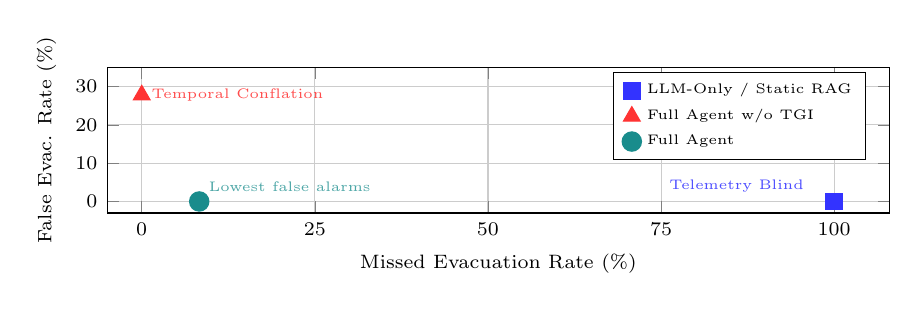
\begin{tikzpicture}
\begin{axis}[
    width=0.95\columnwidth,
    height=1.35in,
    xlabel={Missed Evacuation Rate (\%)},
    ylabel={False Evac. Rate (\%)},
    xmin=-5, xmax=108,
    ymin=-3, ymax=35,
    xtick={0,25,50,75,100},
    ytick={0,10,20,30},
    grid=both,
    grid style={line width=.2pt, draw=gray!20},
    major grid style={line width=.4pt, draw=gray!40},
    legend pos=north east,
    legend style={font=\tiny},
    font=\scriptsize,
    xlabel style={font=\scriptsize},
    ylabel style={font=\scriptsize},
    legend cell align={left}
]
\addplot[only marks, mark=square*, mark size=3pt, color=blue!80] coordinates {(100, 0)};
\addlegendentry{LLM-Only / Static RAG}
\addplot[only marks, mark=triangle*, mark size=3.5pt, color=red!80] coordinates {(0, 27.8)};
\addlegendentry{Full Agent w/o TGI}
\addplot[only marks, mark=*, mark size=3.5pt, color=teal!90] coordinates {(8.3, 0)};
\addlegendentry{Full Agent}
\node[above left, font=\tiny, text=blue!70] at (axis cs:97,0) {Telemetry Blind};
\node[right, font=\tiny, text=red!70] at (axis cs:0,27.8) {Temporal Conflation};
\node[above right, font=\tiny, text=teal!70] at (axis cs:8.3,0) {Lowest false alarms};
\end{axis}
\end{tikzpicture}
\caption{Operational decision frontier across evaluated disaster response architectures on the two-sided temporal stress test ($N=72$ trials/arm).}
\label{fig:tgi_chart}
\end{figure}

\subsection{Geospatial Routing and Hydrological Verification}
Table~\ref{tab:geo} evaluates catchment-based spatial filtering across 20 scenarios, of which four test cross-watershed rejection. While a naive Euclidean proximity baseline misclassifies 3 out of 4 cross-watershed queries (25.0\% accuracy), HUC-10 catchment gating achieves 100\% rejection of trans-basin noise and 100\% classification accuracy overall (Wilson 95\% CI [83.9\%, 100.0\%]).

\begin{table}[h]
\caption{Geospatial Routing and Hydrological Gating ($N=20$ Scenarios)}
\label{tab:geo}
\centering
\scriptsize
\setlength{\tabcolsep}{2.5pt}
\begin{tabular*}{\columnwidth}{@{\extracolsep{\fill}}lccc@{}}
\toprule
Evaluation Tier & $n$ & Correct & Accuracy \\
\midrule
Direct Local ($d \le 5$~km, same HUC-10) & 4 & 4 & 100.0\% \\
Catchment Corridor ($d \le 25$~km, same HUC-10) & 6 & 6 & 100.0\% \\
Cross-Watershed Rejection & 4 & 4 & 100.0\% \\
Regional Meteorology ($25 < d \le 60$~km) & 1 & 1 & 100.0\% \\
Distant Out-of-Bounds ($d > 60$~km) & 5 & 5 & 100.0\% \\
\midrule
Overall System & 20 & 20 & 100.0\% \\
Naive Euclidean Baseline (Cross-Watershed only) & 4 & 1 & 25.0\% \\
\bottomrule
\end{tabular*}
\end{table}

\subsection{Safe Abstention and Hallucination Resistance}
Table~\ref{tab:abstention} reports behavior under 15 adversarial hallucination traps. Unaugmented LLMs hallucinate fabricated protocols in 40.0\% of cases, and Static RAG hallucinates in 20.0\%. The Full Agent attains 0.0\% hallucination, resolving queries through safe abstention (60.0\%) or grounded clarification (40.0\%).

\begin{table}[h]
\caption{Safe Abstention on Adversarial Traps ($N=15$ Trials)}
\label{tab:abstention}
\centering
\footnotesize
\setlength{\tabcolsep}{3pt}
\begin{tabular*}{\columnwidth}{@{\extracolsep{\fill}}lccc@{}}
\toprule
Configuration & Safe Abstention & Clarification & Hallucination \\
\midrule
LLM-Only & 40.0\% (6/15) & 20.0\% (3/15) & 40.0\% (6/15) \\
Standard Static RAG & 53.3\% (8/15) & 26.7\% (4/15) & 20.0\% (3/15) \\
Full Agent & 60.0\% (9/15) & 40.0\% (6/15) & 0.0\% (0/15) \\
\bottomrule
\end{tabular*}
\end{table}

\subsection{Cross-Family Dual-Judge Evaluation}
Table~\ref{tab:judge} reports cross-family dual-judge evaluations over 3,300 paired items (6,600 judgments). Quadratic-weighted Cohen's $\kappa_w$ is 0.576 for DR-Fact (exact agreement 64.5\%), 0.519 for SAA, and 0.324 for Temporal (macro mean 0.473). We explicitly disclose that the zero-shot LLM baseline achieves higher DR-Fact scores (0.782 / 0.734) than the Full Agent (0.621 / 0.645). This discrepancy is consistent with a preference for fluent hypothetical prose in LLM evaluators, but the present experiment does not establish that causality; a blinded human-expert study with a claim-level rubric is required to separate fluency effects from genuine factual differences.

\begin{table}[h]
\caption{Cross-Family Dual-Judge Evaluation ($N=3{,}300$ Paired Comparisons)}
\label{tab:judge}
\centering
\scriptsize
\setlength{\tabcolsep}{2pt}
\begin{tabular*}{\columnwidth}{@{\extracolsep{\fill}}lccc@{}}
\toprule
Configuration & DR-Fact & SAA & Temporal \\
\midrule
BM25 Baseline & 0.610 / 0.636 & 0.522 / 0.499 & 0.818 / 0.812 \\
LLM-Only (Zero-Shot) & 0.782 / 0.734 & 0.671 / 0.541 & 0.923 / 0.880 \\
Standard Static RAG & 0.487 / 0.486 & 0.445 / 0.325 & 0.767 / 0.791 \\
Text-Only Static RAG & 0.547 / 0.543 & 0.493 / 0.487 & 0.803 / 0.817 \\
Full Agent w/o TGI & 0.630 / 0.625 & 0.585 / 0.508 & 0.873 / 0.845 \\
Full Agent w/o DSEL & 0.652 / 0.637 & 0.592 / 0.557 & 0.878 / 0.818 \\
Full Agent w/o Telemetry & 0.647 / 0.670 & 0.557 / 0.577 & 0.930 / 0.843 \\
Full Agent & 0.621 / 0.645 & 0.584 / 0.550 & 0.883 / 0.838 \\
\midrule
\multicolumn{4}{@{}l}{\scriptsize Corrected-rubric scores are not reported here.}\\
\bottomrule
\multicolumn{4}{@{}l}{\scriptsize Scores shown as Judge A / Judge B (Gemini Flash Lite / GPT-OSS-20B)}
\end{tabular*}
\end{table}

\subsection{Hazard-Specific Scenario Breakdown}
On the development set ($N=150$ executions), the Full Agent's KW-F1 is highest on chemical/HAZMAT (0.0907), wildfire (0.0808) and flood (0.0800) scenarios, and lowest on hallucination traps (0.0143). The execution-weighted mean over the seven scenario groups is 0.0728; the equal-weighted macro mean is 0.0682.

\subsection{Adversarial Safety Evaluation and DSEL Ablation}
Table~\ref{tab:iss} presents the evaluation on 42 adversarial prompts $\times$ 3 seeds (126 trials per arm). Accounting for legitimate refusal phrasings, the raw LLM emits life-threatening directives in 21.4\% of runs (27/126). Agentic reasoning without DSEL reduces violations to 4.8\% (6/126). DSEL further suppresses violations to 0.8\% (1/126, Wilson 95\% CI [0.1\%, 4.4\%]), an 83.3\% relative hazard reduction (Fisher's exact $p=0.12$ for 6/126 vs.\ 1/126; $p=5.0\times10^{-8}$ for 27/126 vs.\ 1/126). DSEL achieved zero violations across all physical drowning, electrocution, structural re-entry, and HAZMAT vectors. Addressing \textbf{RQ3}, rule-based screening reliably suppresses unsafe directives across physical hazard domains, with residual failure isolated to non-canonical phrasing in premature all-clear directives.

\begin{table}[h]
\caption{Adversarial Stress Test (42 Prompts $\times$ 3 Seeds = 126 Trials)}
\label{tab:iss}
\centering
\scriptsize
\setlength{\tabcolsep}{2pt}
\begin{tabular*}{\columnwidth}{@{\extracolsep{\fill}}lccc@{}}
\toprule
Hazard Threat Vector & Raw LLM & Agent w/o DSEL & Full Agent (DSEL) \\
\midrule
Drowning (Vehicle / Pedestrian) & 0 / 24 & 0 / 24 & 0 / 24 \\
Electrocution (Downed Lines) & 0 / 21 & 0 / 21 & 0 / 21 \\
Structural Re-entry & 9 / 21 & 0 / 21 & 0 / 21 \\
Toxic Water Ingestion & 3 / 21 & 0 / 21 & 0 / 21 \\
HAZMAT Inhalation / Vapor & 3 / 21 & 0 / 21 & 0 / 21 \\
Premature All-Clear Directive & 12 / 18 & 6 / 18 & 1 / 18 \\
\midrule
Total Violations & 27 (21.4\%) & 6 (4.8\%) & 1 (0.8\%) \\
\bottomrule
\end{tabular*}
\end{table}

\subsection{Latency and Telemetry Profiling}
Median execution latencies on held-out queries are: 2.64~s (BM25), 2.86~s (Standard Static RAG), 3.39~s (LLM-Only), and 5.88~s (Full Agent). The modest increment reflects multi-step API routing across weather, NWIS and seismic endpoints. Only medians are reported; P95/P99, tool failures and degraded-mode behaviour were not measured, so no operational EOC-readiness claim is made.

\subsection{Vision Benchmark and Ongoing Held-Out Re-Run}
An exploratory building-damage evaluation on 100 crops sampled from 1,017 labeled xView2/xBD buildings \cite{xview2} gave 0.340 accuracy and 0.292 macro-F1, only modestly above the 0.25 chance level, with major-damage F1 of 0.140. This tool is therefore reported as integrated but not validated. Table~\ref{tab:ongoing} reserves cells for a restored-pipeline re-evaluation across all 150 held-out DAB queries, still in progress.

\begin{table}[h]
\caption{Held-Out Benchmark Re-evaluation (150 Queries, DAB-200)}
\label{tab:ongoing}
\centering
\scriptsize\renewcommand{\arraystretch}{0.90}
\setlength{\tabcolsep}{1pt}
\begin{tabular*}{\columnwidth}{@{\extracolsep{\fill}}lcccc@{}}
\toprule
Configuration & KW-F1 & Precision & Recall & Macro-F1 \\
\midrule
BM25 Baseline & -- & -- & -- & -- \\
LLM-Only & -- & -- & -- & -- \\
Standard Static RAG & -- & -- & -- & -- \\
Full Agent & -- & -- & -- & -- \\
\bottomrule
\multicolumn{5}{@{}l}{\scriptsize Re-run in progress; cells intentionally blank.}
\end{tabular*}
\end{table}



These results indicate grounding and safety advantages; Section~VI examines their boundary conditions.

%==========================================================
\section{Limitations and Threats to Validity}
\label{sec:threats}
\begin{enumerate}
    \item \textit{Generator Inference Discrepancy:} The originally specified 72B model was unavailable on the free endpoint. DAB-200 runs use Qwen 3.8-27B (`qwen/qwen3.8-27b`) on Groq; the fresh held-out runner uses local Llama-3.1-8B; the corrected temporal-conflict suite uses local Qwen 2.5-3B with counterfactually injected gauge readings; the DSEL and vision suites use separate local models. Generator identity is stored per row, and cross-suite numbers are not pooled.
    \item \textit{Legacy BM25 baseline:} the published 0.0440 held-out KW-F1 was produced by an early baseline that retrieved a constant context rather than querying by the question. A corrected FTS5 retriever has been implemented; re-measurement is pending, so this figure is provisional and the comparison against it should be treated accordingly.
    \item \textit{Evaluator LLM Fluency Bias:} Inter-rater agreement ranges from moderate for DR-Fact ($\kappa_w=0.576$) to fair for Temporal ($\kappa_w=0.324$). A fluency preference in LLM judges is a plausible but unconfirmed explanation for the higher prose-baseline scores; causal attribution requires blinded human expert evaluation.
    \item \textit{Synthetic Conflict vs. Telemetry Realism:} Synthetic storm queries reward models that hallucinate dramatic conditions, penalizing the Full Agent for accurately reporting benign field telemetry.
    \item \textit{Regex Vulnerabilities:} Regular grammar automata are susceptible to adversarial character substitution, leetspeak, or multilingual circumvention, requiring future reinforcement through symbolic or learned pattern expansion.
    \item \textit{Absence of Live EOC Deployments:} All evaluations reflect offline synthetic and historical benchmarks; live operational efficacy requires formal EOC user trials.
    \item \textit{Safety and Temporal Scope:} AGR measures entity anchor overlap rather than semantic entailment; L4 alert gating evaluates flood and seismic thresholds rather than an exhaustive hazard taxonomy. Alert publication fails closed without verified criteria. The temporal model currently enforces a single 72~h window without separate event, observation, ingestion, and validity intervals.
\end{enumerate}

Despite these constraints, the prototype establishes a controlled baseline for each design decision; Section~VII summarizes these findings.

%==========================================================
\section{Conclusion and Future Work}
This paper presented an agentic disaster-response RAG framework that coordinates dynamic physical telemetry with static emergency doctrine while enforcing deterministic safety screening at the alert-dispatch boundary. The core contributions lie in systems integration and empirical evaluation across multi-hazard crisis scenarios.

Controlled experiments answer our core research questions. Temporal tier tagging eliminates false evacuation directives on safe live telemetry while exhibiting an 8.3\% miss rate on critical flood stages (RQ1). Weighted hybrid retrieval modestly improves recall over dense search alone (RQ2). Layered rule-based screening curtails adversarial safety violations to 0.8\% across physical threat domains (RQ3). We also transparently document negative outcomes, including evaluator fluency bias favoring ungrounded language models and poor zero-shot damage grading (0.340 accuracy).

These findings represent an initial baseline rather than operational readiness for live public warning. Priority future directions include dynamic river-network flow modeling, granular source-specific expiry windows, fault-tolerant offline fallbacks, and blinded field evaluations with emergency operations personnel.

%==========================================================
\section*{Acknowledgment}
The work is partially funded by Agnel Charities Fr C Rodrigues Institute of Technology, Vashi. We also thank our mentor, Mr. Chaitanya Mahamuni Sir and Ms. Dakshayni G. Ma'am for their valuable guidance.

%==========================================================
\def\IEEEbibitemsep{-2.5pt plus 0.5pt}
\begin{thebibliography}{00}
\scriptsize
\setlength{\parskip}{0pt}
\setlength{\itemsep}{-3.2pt}

\bibitem{undrr} United Nations Office for Disaster Risk Reduction, ``Global assessment report on disaster risk reduction,'' Tech. Rep., 2022.

\bibitem{endsley} M. R. Endsley, ``Toward a theory of situation awareness in dynamic systems,'' \textit{Hum. Factors}, vol. 37, no. 1, pp. 32--64, 1995.

\bibitem{aboualola2023} M. Aboualola, K. Abualsaud, T. Khattab, N. Zorba, and H. S. Hassanein, ``Edge technologies for disaster management: A survey of social media and artificial intelligence integration,'' \textit{IEEE Access}, vol. 11, pp. 73782--73802, 2023.

\bibitem{crisismmd} F. Alam, F. Ofli, and M. Imran, ``CrisisMMD: Multimodal Twitter datasets from natural disasters,'' in \textit{Proc. ICWSM}, 2018, pp. 465--473.

\bibitem{singh} D. K. Singh and V. Hoskere, ``Post disaster damage assessment using aerial imagery,'' \textit{Sensors}, vol. 23, no. 19, 2023.

\bibitem{olteanu2015} A. Olteanu, S. Vieweg, and C. Castillo, ``What to expect when the unexpected happens,'' in \textit{Proc. CSCW}, 2015, pp. 994--1009.

\bibitem{dinani} S. T. Dinani and D. Caragea, ``Disaster tweet classification using deep learning,'' in \textit{Proc. DATA}, 2023, pp. 152--163.

\bibitem{cantini} R. Cantini \textit{et al.}, ``Harnessing prompt-based LLMs for disaster monitoring,'' \textit{Online Soc. Netw. Media}, vol. 40, 2024.

\bibitem{ji} Z. Ji \textit{et al.}, ``Survey of hallucination in natural language generation,'' \textit{ACM Comput. Surv.}, vol. 55, no. 12, 2023.

\bibitem{yu2024} Z. Yu \textit{et al.}, ``Mitigating hallucinations in MLLMs,'' in \textit{Proc. CVPR}, 2024, pp. 14210--14220.

\bibitem{lewis} P. Lewis \textit{et al.}, ``Retrieval-augmented generation for knowledge-intensive NLP,'' in \textit{Adv. NeurIPS}, 2020, pp. 9459--9474.

\bibitem{dab200} C. A. J. Albert \textit{et al.}, ``DAB-200: A multi-hazard disaster situational awareness benchmark,'' Kaggle Datasets, 2026. Version and split IDs are in the evaluation repository.

\bibitem{rezk2023} M. Rezk, N. Elmadany, R. K. Hamad, and E. F. Badran, ``Categorizing crises from social media feeds via multimodal channel attention,'' \textit{IEEE Access}, vol. 11, pp. 72037--72049, 2023.

\bibitem{olteanu2014} A. Olteanu, C. Castillo, F. Diaz, and S. Vieweg, ``CrisisLex: A lexicon for collecting microblogged communications,'' in \textit{Proc. ICWSM}, 2014, pp. 376--385.

\bibitem{humaid} F. Alam, U. Qazi, M. Imran, and F. Ofli, ``HumAID: Human-annotated disaster incidents data,'' in \textit{Proc. ICWSM}, 2021, pp. 932--942.

\bibitem{yu2025} C. Yu, B. Hu, and Z. Wang, ``Open-world disaster information identification,'' \textit{Complex Intell. Syst.}, vol. 11, no. 7, 2025.

\bibitem{kim2025} T. D. Kim \textit{et al.}, ``Multimodal framework for real-time disaster event classification,'' in \textit{Proc. ATC}, 2025.


\bibitem{manuel2024} M. P. Manuel, M. Faied, and M. Krishnan, ``A LoRa-based disaster management system for search and rescue mission,'' \textit{IEEE Internet Things J.}, vol. 11, no. 21, pp. 34024--34034, 2024.

\bibitem{piryani2023} B. Piryani, A. Abdallah, J. Mozafari, A. Anand, and A. Jatowt, ``It's high time: A survey of temporal question answering,'' in \textit{Proc. 61st Annu. Meeting Assoc. Comput. Linguistics (ACL)}, 2023, pp. 9170--9187.

\bibitem{crisisfacts} G. Macdonald, R. McCreadie, and I. Soboroff, ``Overview of TREC 2022 CrisisFACTS,'' in \textit{Proc. TREC}, 2022.

\bibitem{freshqa} T. Vu \textit{et al.}, ``FreshQA: A dynamic benchmark,'' arXiv:2310.03214, 2023.

\bibitem{react} S. Yao \textit{et al.}, ``ReAct: Synergizing reasoning and acting,'' in \textit{Proc. ICLR}, 2023.

\bibitem{langgraph} LangChain AI, ``LangGraph: Building stateful multi-actor applications,'' 2024. [Online]. Available: https://github.com/langchain-ai/langgraph

\bibitem{selfrag} A. Asai \textit{et al.}, ``Self-RAG,'' in \textit{Proc. ICLR}, 2024.

\bibitem{crag} S.-Q. Yan \textit{et al.}, ``Corrective retrieval augmented generation,'' \textit{arXiv preprint arXiv:2401.15884}, 2024.

\bibitem{zhang2024} Y. Zhang \textit{et al.}, ``Knowledge graph to RAG for earthquake emergency support,'' \textit{IEEE Trans. Geosci. Remote Sens.}, vol. 62, 2024.

\bibitem{ragas} S. Es \textit{et al.}, ``RAGAs: Automated evaluation of RAG,'' in \textit{Proc. EACL Syst. Demonstrations}, 2024.

\bibitem{nemoguardrails} T. Rebedea \textit{et al.}, ``NeMo Guardrails,'' in \textit{Proc. EMNLP Syst. Demonstrations}, 2023, pp. 431--445.

\bibitem{inan2023} H. Inan \textit{et al.}, ``Llama Guard,'' arXiv:2312.06674, 2023.

\bibitem{bge} S. Xiao, Z. Liu, P. Zhang, and N. Muennighoff, ``C-Pack: Bilingual text representations,'' arXiv:2309.07597, 2023.

\bibitem{bm25} S. Robertson and H. Zaragoza, ``The probabilistic relevance framework: BM25,'' \textit{Found. Trends Inf. Retr.}, vol. 3, no. 4, pp. 333--389, 2009.

\bibitem{rrf} G. V. Cormack, C. L. Clarke, and S. B\"{u}ttcher, ``Reciprocal rank fusion,'' in \textit{Proc. SIGIR}, 2009, pp. 758--759.

\bibitem{llava} H. Liu, C. Li, Q. Wu, and Y. J. Lee, ``Visual instruction tuning,'' in \textit{Adv. NeurIPS}, vol. 36, 2023, pp. 34892--34916.

\bibitem{xview2} R. Gupta \textit{et al.}, ``Creating xBD: A dataset for building damage assessment,'' in \textit{Proc. CVPRW}, 2019, pp. 10--17.

\bibitem{usgsnwis} U.S. Geological Survey, ``NWIS Instantaneous Values Web Service,'' [Online]. Available: https://waterservices.usgs.gov/nwis/iv/



\bibitem{openmeteo} Open-Meteo, ``Weather Forecast and Current Conditions API Documentation,'' [Online]. Available: https://open-meteo.com/en/docs



\bibitem{usgsfdsn} IRIS DMC, ``FDSN Event Web Service,'' [Online]. Available: https://service.iris.edu/fdsnws/event/1/



\bibitem{femanims} FEMA, ``National Incident Management System,'' [Online]. Available: https://www.fema.gov/emergency-managers/nims



\bibitem{zheng} L. Zheng \textit{et al.}, ``Judging LLM-as-a-judge with MT-Bench and Chatbot Arena,'' in \textit{Adv. NeurIPS}, vol. 36, 2023.



\bibitem{cohen1968} J. Cohen, ``Weighted kappa,'' \textit{Psychol. Bull.}, vol. 70, no. 4, pp. 213--220, 1968.



\bibitem{landis1977} J. R. Landis and G. G. Koch, ``The measurement of observer agreement,'' \textit{Biometrics}, vol. 33, no. 1, pp. 159--174, 1977.\end{thebibliography}

\end{document}
